%\documentclass[handout]{beamer}
\documentclass{beamer}
\usepackage[utf8]{inputenc}
%\usepackage[czech]{babel}

\renewcommand{\O}{\mathcal{O}}

\mode<presentation> {
%\usetheme{default}
%\usetheme{AnnArbor}
%\usetheme{Antibes}
%\usetheme{Bergen}
%\usetheme{Berkeley}
%\usetheme{Berlin}
%\usetheme{Boadilla}
%\usetheme{CambridgeUS}
%\usetheme{Copenhagen}
%\usetheme{Darmstadt}
%\usetheme{Dresden}
%\usetheme{Frankfurt}
%\usetheme{Goettingen}
%\usetheme{Hannover}
%\usetheme{Ilmenau}
%\usetheme{JuanLesPins}
%\usetheme{Luebeck}
\usetheme{Madrid}
%\usetheme{Malmoe}
%\usetheme{Marburg}
%\usetheme{Montpellier}
%\usetheme{PaloAlto}
%\usetheme{Pittsburgh}
%\usetheme{Rochester}
%\usetheme{Singapore}
%\usetheme{Szeged}
%\usetheme{Warsaw}

%\usecolortheme{albatross}
%\usecolortheme{beaver}
%\usecolortheme{beetle}
%\usecolortheme{crane}
%\usecolortheme{dolphin}
%\usecolortheme{dove}
%\usecolortheme{fly}
%\usecolortheme{lily}
%\usecolortheme{orchid}
%\usecolortheme{rose}
%\usecolortheme{seagull}
%\usecolortheme{seahorse}
%\usecolortheme{whale}
%\usecolortheme{wolverine}

%\setbeamertemplate{footline} % To remove the footer line in all slides uncomment this line
%\setbeamertemplate{footline}[page number] % To replace the footer line in all slides with a simple slide count uncomment this line

%\setbeamertemplate{navigation symbols}{} % To remove the navigation symbols from the bottom of all slides uncomment this line
}

\usepackage{graphicx} % Allows including images
\usepackage{booktabs} % Allows the use of \toprule, \midrule and \bottomrule in tables

%----------------------------------------------------------------------------------------
%	TITLE PAGE
%----------------------------------------------------------------------------------------

\title{Scalable link-time optimization} % The short title appears at the bottom of every slide, the full title is only on the title page

\author{Ladislav Láska} % Your name
\institute[MFF UK] % Your institution as it will appear on the bottom of every slide, may be shorthand to save space
{
Faculty of Mathematics and Physics, Charles University \\ % Your institution for the title page
\medskip
\texttt{laska@kam.mff.cuni.cz} % Your email address
}
\date{\today} % Date, can be changed to a custom date

\begin{document}

\begin{frame}
\titlepage % Print the title page as the first slide
\end{frame}

%------------------------------------------------
\section{First Section} % Sections can be created in order to organize your presentation into discrete blocks, all sections and subsections are automatically printed in the table of contents as an overview of the talk
%------------------------------------------------


\begin{frame}[t]
	\frametitle{What is link-time optimization (LTO)?}
	\begin{itemize}
		\item<1-> Programs are composed of many source files ({\it
			compilation units}).
		\item<1-> Each unit is compiled and optimized separately, all of them are
			linked together to form a single binary.
		\item<2-> We can perform further optimizations at link-time.
	\end{itemize}
	\centering
	\only<1>{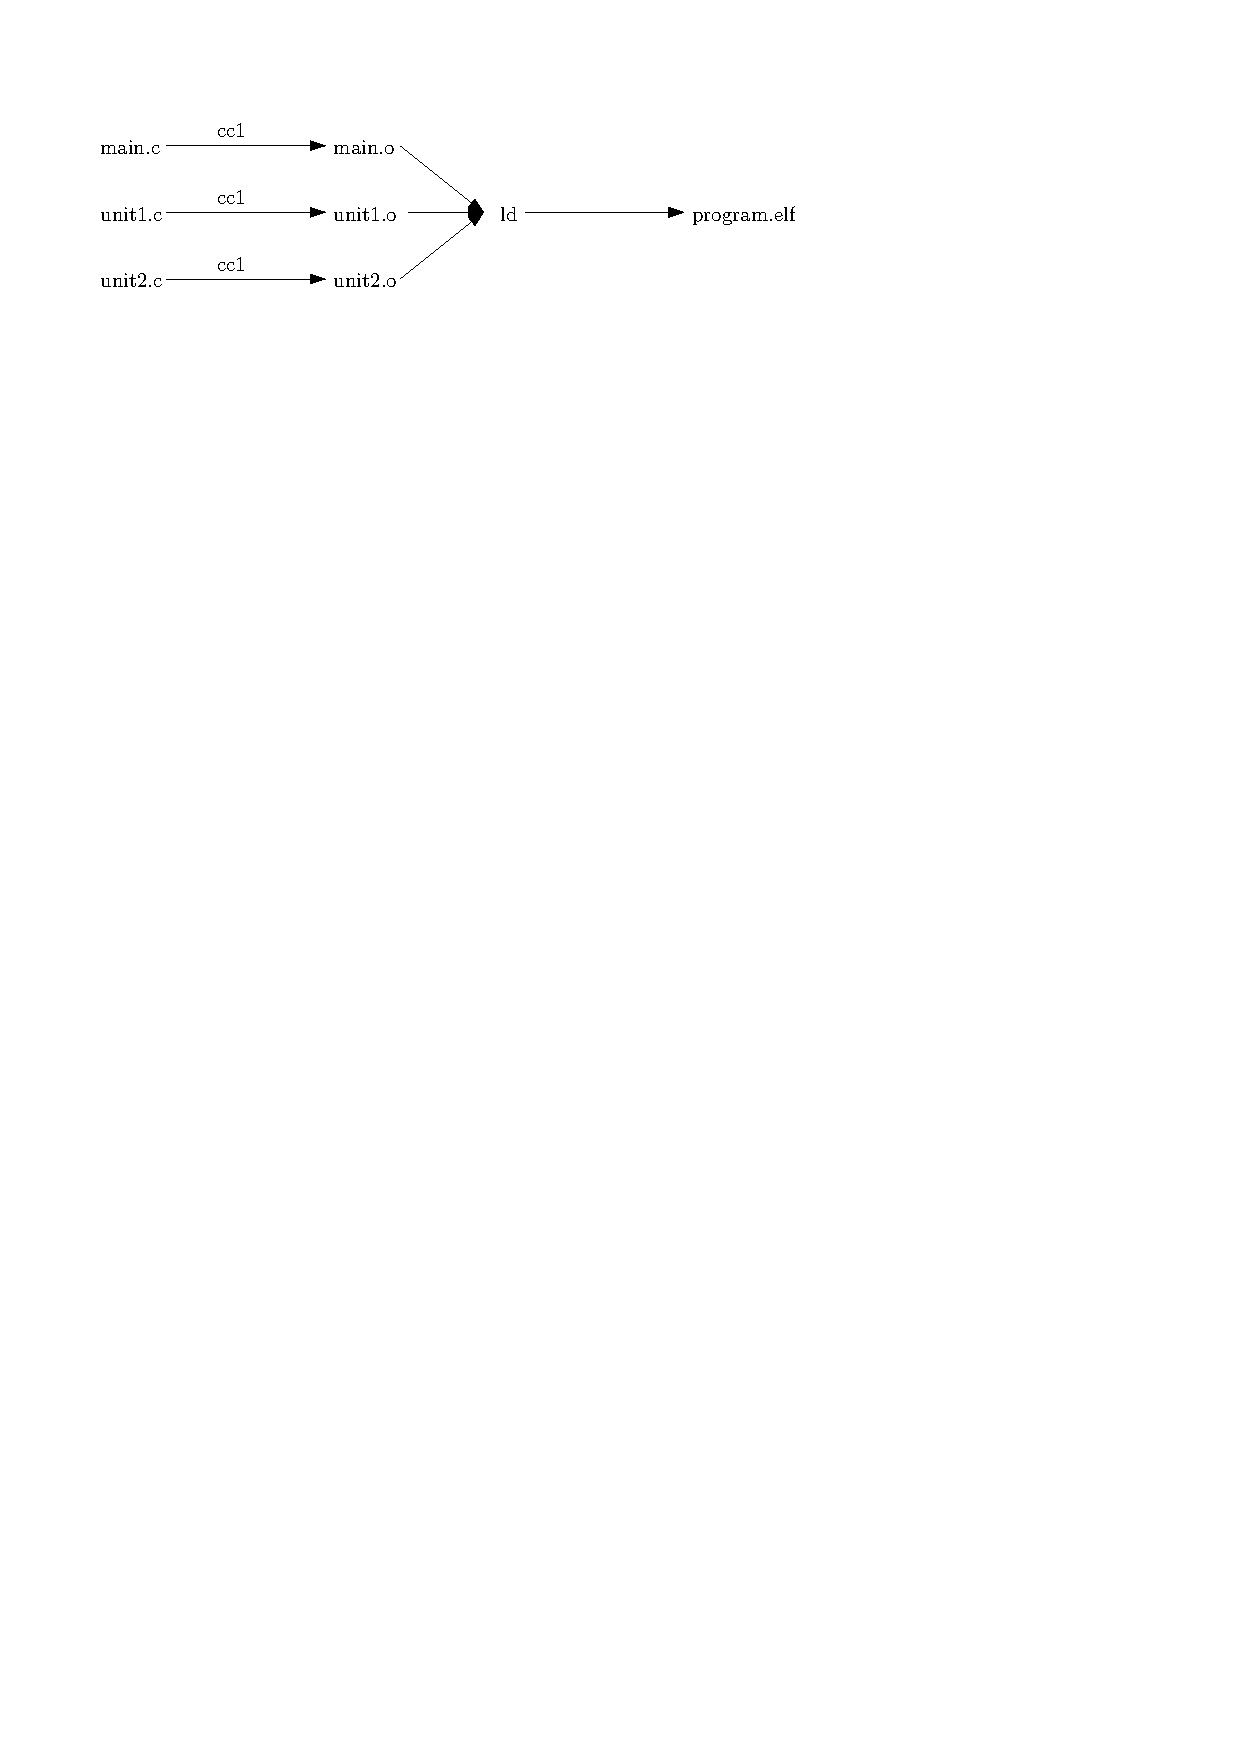
\includegraphics[width=0.7\textwidth]{../img/non-lto-workflow.pdf}}
	\only<2>{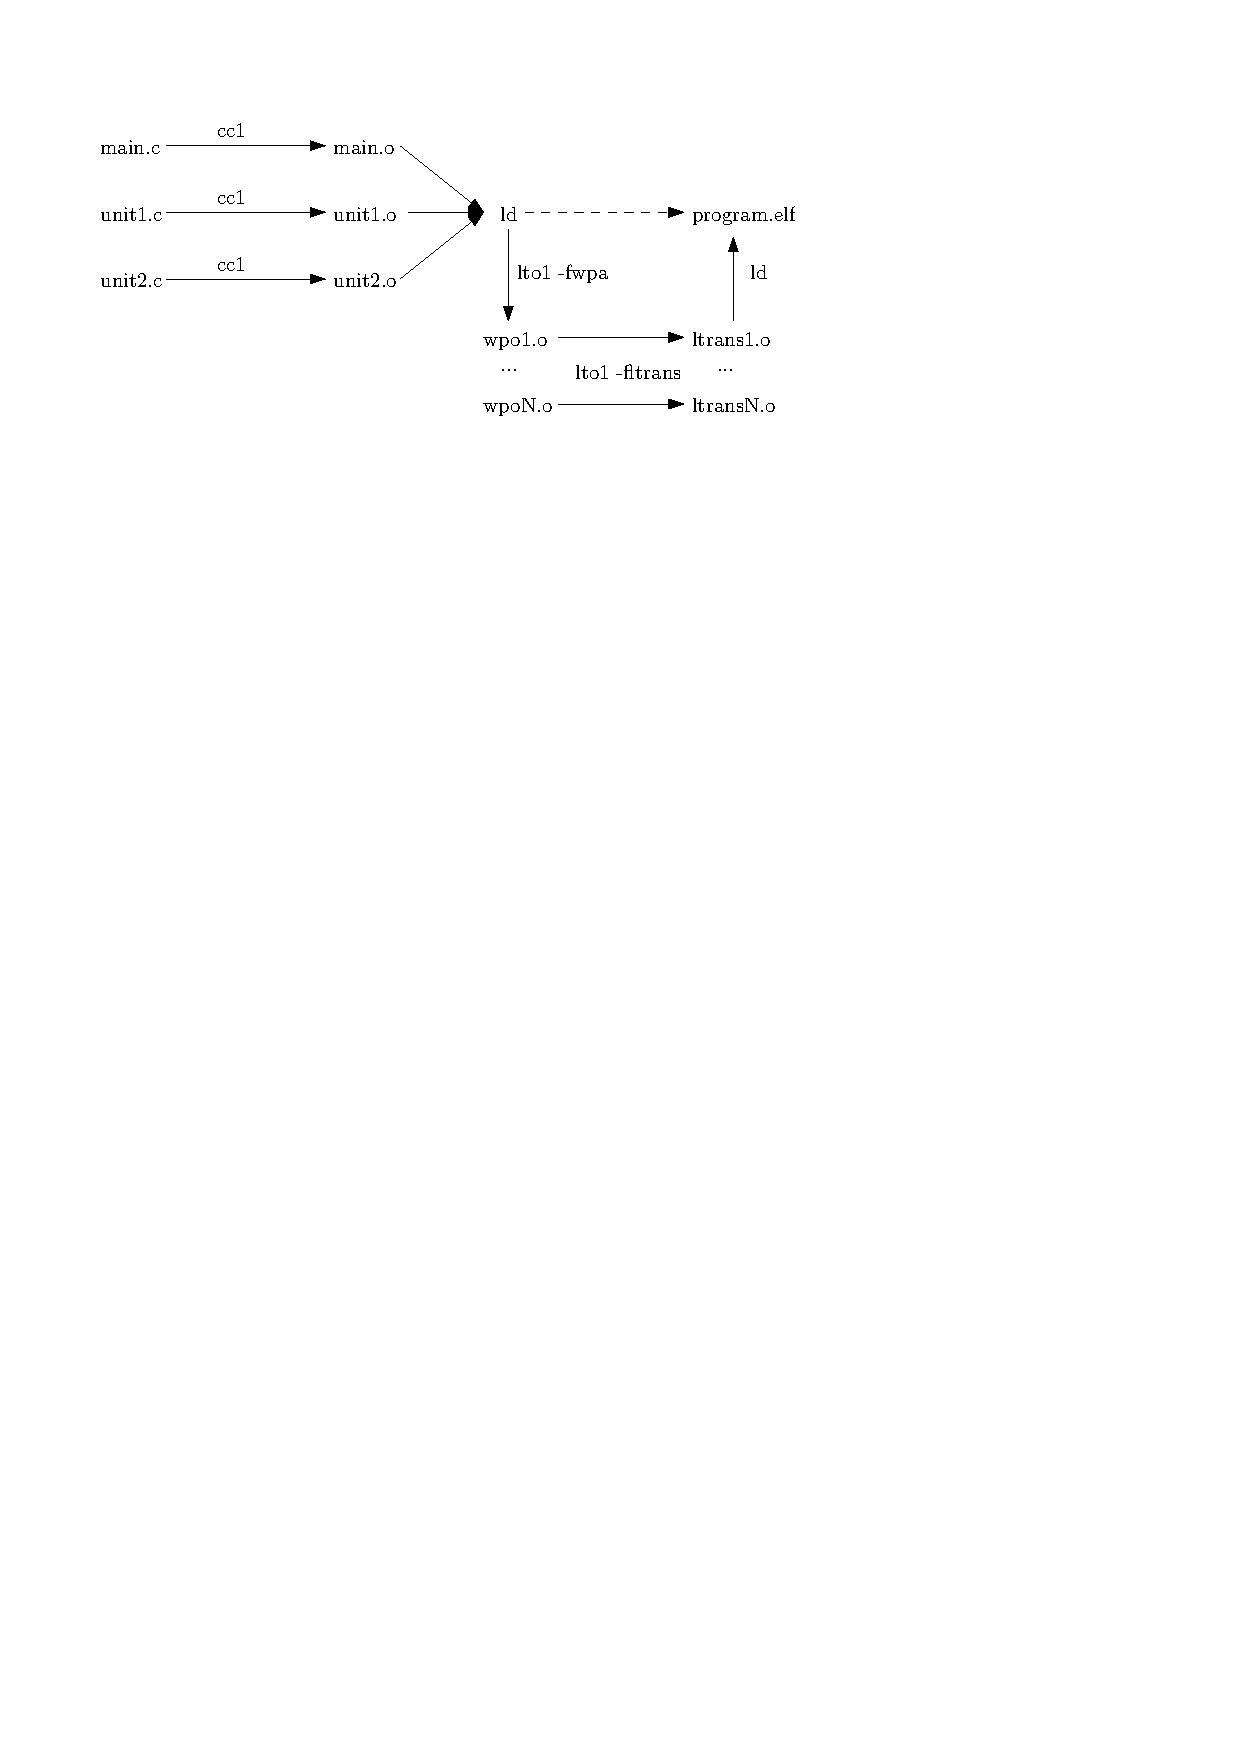
\includegraphics[width=0.7\textwidth]{../img/lto-workflow.pdf}}
\end{frame}

\begin{frame}[t]
\frametitle{What is link-time optimization (LTO)?}
\textbf{Requirements}
\begin{itemize}
	\item Programmers like readable code, categorized by their function.
	\item Compilers need as much information as possible to optimize.
\end{itemize}
\pause
\vfill
\textbf{Benefits} 
\begin{itemize}
	\item Programmers have less need to optimize manually.
	\item Many inter-unit optimizations are possible, for example:
		\begin{itemize}
			\item Constant propagation.
			\item Inlining.
			\item Devirtualization.
		\end{itemize}
\end{itemize}
\end{frame}


%------------------------------------------------

\begin{frame}[t]
\frametitle{Difficulties}
\begin{itemize}
		\item<1-> There are some large programs that need optimizing, growing every
			year.

		\only<1>{\centering\includegraphics[width=0.6\textwidth]{../graphs/loc/loc.pdf}}
		\item<2-> The code is usually linked into a single library.

		\only<2>{\hspace{1.5cm}\includegraphics[angle=-90,trim=0 30 10 0,clip,width=0.6\textwidth]{../graphs/firefox-objsize/objsize.pdf}}
		
		\item<3-> Some optimization techniques do not scale well.
\end{itemize}
\end{frame}

%------------------------------------------------

\begin{frame}[t]
	\frametitle{Compiling Firefox using GCC}
	\begin{itemize}
		\item {Whole Firefox, no LTO.}

			{\hspace{1.5cm}\includegraphics[width=0.6\textwidth]{../graphs/firefox-nolto/firefox-ipa-pta.pdf}}

		\pause
		\item {{\tt libxul.so} with {\tt -flto=8}}

			{\hspace{1.5cm}\includegraphics[width=0.6\textwidth]{../graphs/firefox-lto8/firefox-ipa-pta.pdf}}

	\end{itemize}
\end{frame}

%------------------------------------------------

\begin{frame}[t]
	\frametitle{Compiling Firefox using GCC}
	\begin{itemize}
		\item {{\tt libxul.so} with {\tt -fipa-pta -flto=8}}

			{\hspace{1.5cm}\includegraphics[width=0.6\textwidth]{../graphs/firefox-ipa-pta-lto8/firefox-ipa-pta.pdf}}

		\pause
		\item {{\tt libxul.so} with {\tt -fipa-pta -flto=2}}

			{\hspace{1.5cm}\includegraphics[width=0.6\textwidth]{../graphs/firefox-ipa-pta-lto2/firefox-ipa-pta.pdf}}

	\end{itemize}
\end{frame}

%------------------------------------------------

\begin{frame}[t]
\frametitle{Interprocedural Points-To Analysis}
\begin{itemize}
	\item The {\tt IPA-PTA} computes interprocedural alias information.
	\item It implements an Andersen-style algorithm, iteratively solving
		constraints induced by pointer operations.
		\pause
		\begin{align*}
			\tag{inititialization}
			p_i = \&a \quad &\to \quad a \in p_i \\
			\tag{copy}
			p_i = p_j \quad &\to \quad p_j \subseteq p_i \\
			\tag{dereference}
			p_i = *p_j \quad &\to \quad \forall p_k \in p_j : p_k \subseteq p_i
		\end{align*}
	\pause
	\item Dereferences are translated into copy constraints as discovered.
	\pause
	\item Copy constrains are implemented as {\it set union}.
	\pause
	\item Points-to sets are currently implemented as bitmaps.
\end{itemize}
\end{frame}

%------------------------------------------------

\begin{frame}[t]
\frametitle{Interprocedural Points-To Analysis}
\begin{itemize}
	\item<1-> Points-to sets are currently implemented as bitmaps.

\centering
\only<1>{
    \textbf{10 most used function during compilation} (without IPA-PTA)
		\bigskip
	\begin{tabular}{|c|l|l|}\hline Overhead & Cmd/Object & Symbol \\  \hline
\hline$2.92\%$ & \tt ltrans\hfill/lto1 & \tt bitmap\_set\_bit \\
\hline $2.19\%$ & \tt ltrans\hfill/libc & \tt \_int\_malloc \\
\hline $1.92\%$ & \tt ltrans\hfill/lto1 & \tt bitmap\_clear\_bit \\
\hline $1.40\%$ & \tt ltrans\hfill/lto1 & \tt ggc\_internal\_alloc \\
\hline $1.26\%$ & \tt ltrans\hfill/lto1 & \tt record\_reg\_classes \\
\hline $1.16\%$ & \tt ltrans\hfill/lto1 & \tt process\_bb\_lives \\
\hline $1.07\%$ & \tt ltrans\hfill/lto1 & \tt df\_note\_compute \\
\hline $0.91\%$ & \tt ltrans\hfill/lto1 & \tt bitmap\_bit\_p \\
\hline $0.91\%$ & \tt ltrans\hfill/lto1 & \tt df\_ref\_create\_structure \\
\hline $0.88\%$ & \tt wpa\hfill/lto1 & \tt inflate\_fast \\
\hline \end{tabular}

	}
\only<2>{
    \textbf{10 most used function during compilation} (with IPA-PTA)
		\bigskip
	\begin{tabular}{|c|l|l|}\hline Overhead & Cmd/Object & Symbol \\  \hline
\hline $80.99\%$ & \tt ltrans\hfill/lto1 & \tt bitmap\_ior\_into \\
\hline $3.62\%$ & \tt ltrans\hfill/lto1 & \tt bitmap\_set\_bit \\
\hline $2.11\%$ & \tt ltrans\hfill/lto1 & \tt find\_what\_var\_points\_to \\
\hline $1.79\%$ & \tt ltrans\hfill/lto1 & \tt do\_complex\_constraint \\
\hline $0.53\%$ & \tt ltrans\hfill/lto1 & \tt find \\
\hline $0.40\%$ & \tt ltrans\hfill/lto1 & \tt bitmap\_copy \\
\hline $0.38\%$ & \tt ltrans\hfill/lto1 & \tt bitmap\_bit\_p \\
\hline $0.36\%$ & \tt ltrans\hfill/lto1 & \tt bitmap\_elt\_insert\_after \\
\hline $0.35\%$ & \tt ltrans\hfill/lto1 & \tt add\_graph\_edge \\
\hline $0.34\%$ & \tt ltrans\hfill/lto1 & \tt solve\_constraints \\
\hline \end{tabular}

	}
	\item<3-> Set union/bitmap operations are a significant bottleneck.
	\item<4-> Improving bitmaps will prove useful in other partos of GCC as
		well.
	\item<5-> There are a few interesting alternatives:
		\begin{itemize}
			\item Binary decision diagrams,
			\item Bloom filters,
			\item Ebitmaps,
			\item and others.
		\end{itemize}
\end{itemize}

\end{frame}

%------------------------------------------------

\begin{frame}[t]
\frametitle{Bloom filters}
\begin{itemize}
		\item A compact probabilistic data structure.
		\begin{itemize}
			\item Size depends only on expected number of elements and
				acceptable probabilitty of {\it false-positive}.
			\item {\tt INSERT}, {\tt QUERY} in $\mathcal{O}(1)$ time.
			\item {\tt UNION}, {\tt BITWISE\_INTERSECTION} in $\mathcal{O}(m)$ time.
			\item {\tt DELETE}, {\tt ENUMERATE}, {\tt RESIZE} not supported.
		\end{itemize}
		\pause
	\item {\tt UNION} can be implemented using bitwise {\tt OR}.
		\pause
	\item False-positives are not a problem, as long as we generate
		conservatively correct answers.
		\pause
	\item Unsupported {\tt ENUMERATE} is a problem, we need it for dereferences.
\end{itemize}
\end{frame}

%------------------------------------------------

\begin{frame}[t]
\frametitle{Bloomaps}
\begin{itemize}
		\item Bloom filters grouped into families, set operations supported only
			inside family.
		\pause
		\item Family supports {\tt NUMERATE} on any Bloomap in $\mathcal{O}(N)$
			time worst-case.
		\pause
		\item Elements inserted into Bloomaps are indexed in Family, allowing
			for faster enumeration.
		\pause
		\item Extra memory is allocated for each family to hold the index.
\end{itemize}
\end{frame}

%------------------------------------------------

\begin{frame}[t]
\frametitle{Bloomaps}


	\centering{

		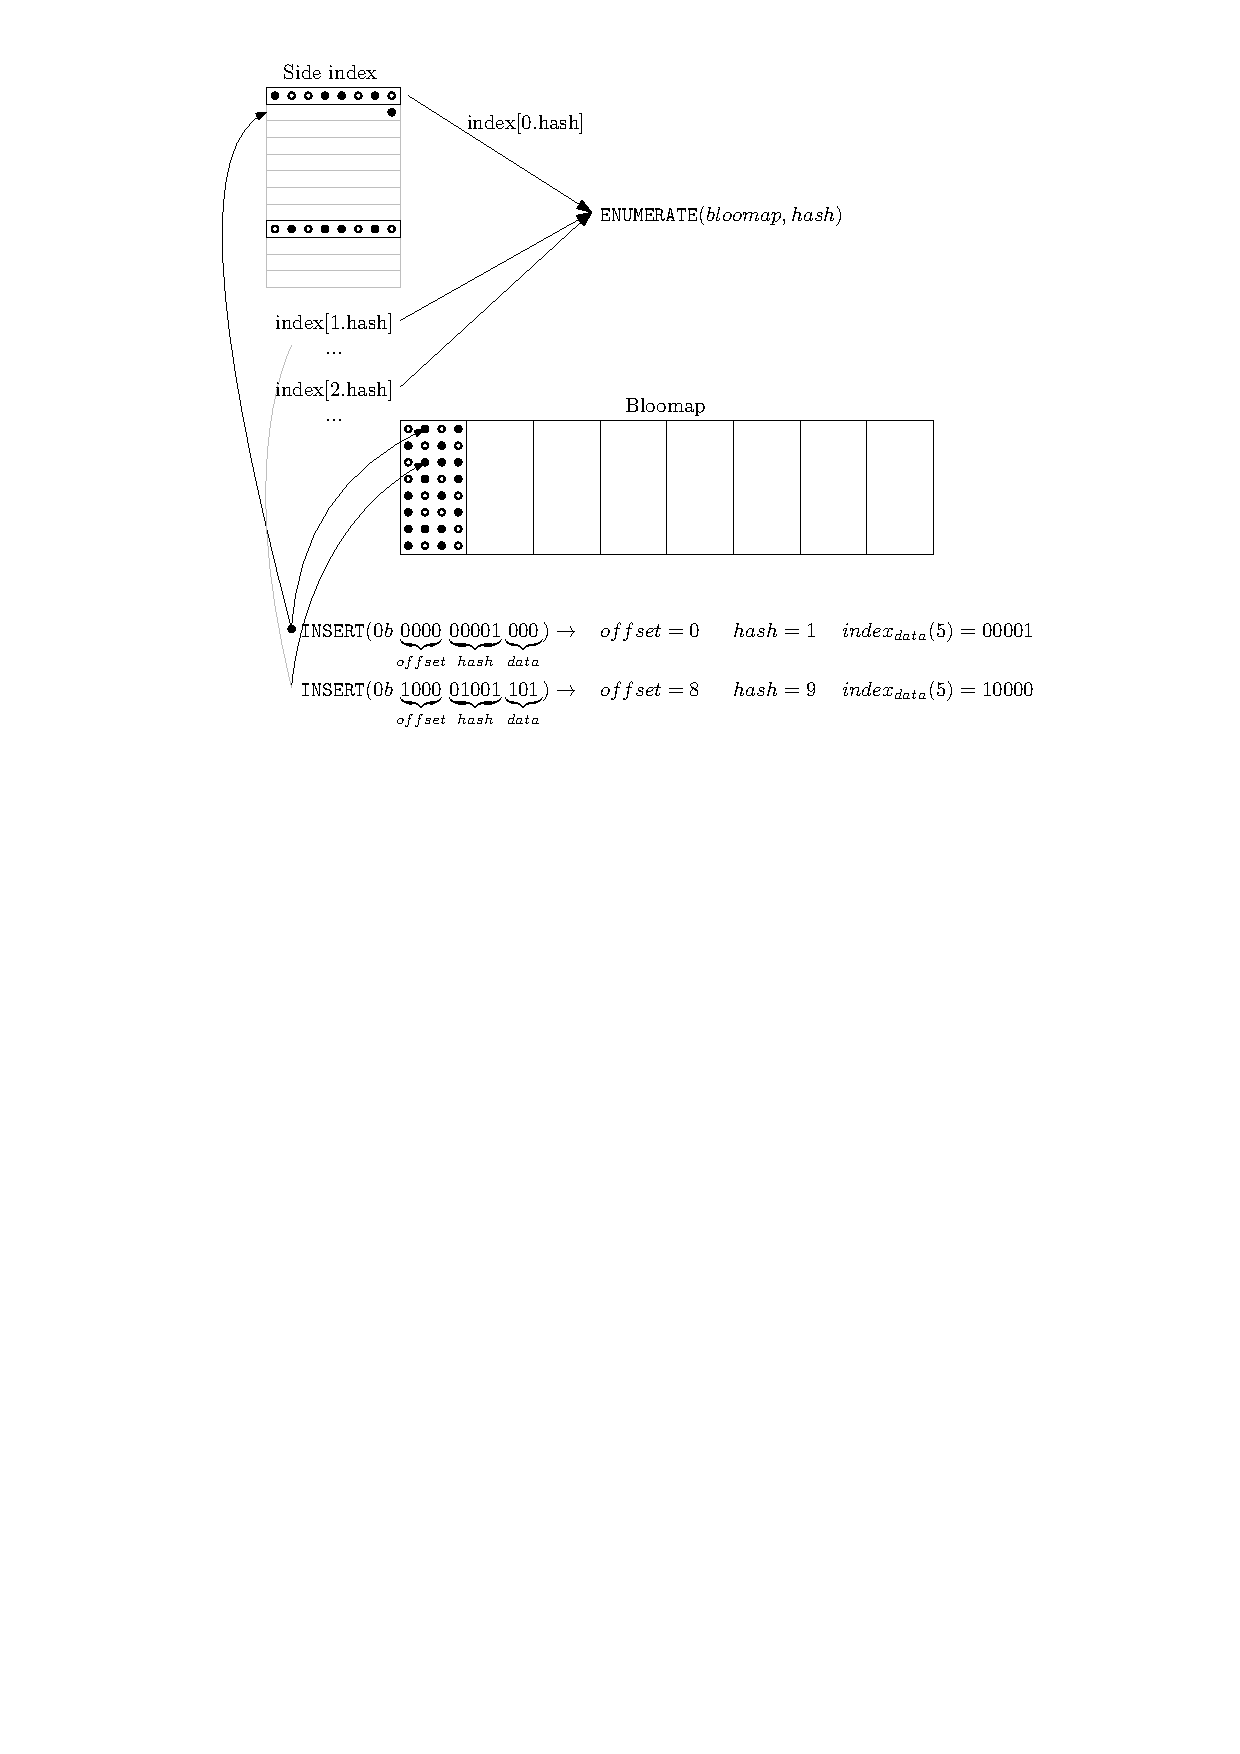
\includegraphics[width=0.7\textwidth]{../img/bloomap_overview.pdf}
	}


\end{frame}
%------------------------------------------------

\begin{frame}[t]
\frametitle{Bloomaps performance}
	\begin{itemize}
		\item {\tt INSERT} adds $\O(1)$ to insert into Family index.
		\item {\tt UNION} adds $\O(1)$ to check if Bloomaps belong to same
			family.
		\item With Bloomaps configured for $1\%$ false-positive rate, the
			results are within $2\%$ of exact data structure.
		\item GCC no longer spends all its time in bitmap functions.
	\end{itemize}
\end{frame}

\begin{frame}[t]
\frametitle{Bloomaps performance}
	\centering{
    \textbf{10 most used function during compilation} (with IPA-KPTA)
	\bigskip

	\begin{tabular}{|c|l|l|}\hline Overhead & Cmd/Object & Symbol \\  \hline
\hline$4.22\%$ & \tt ltrans\hfill/lto1 & \tt bitmap\_find\_bit \\
\hline $1.32\%$ & \tt ltrans\hfill/lto1 & \tt bitmap\_set\_bit \\
\hline $1.15\%$ & \tt ltrans\hfill/lto1 & \tt bitmap\_clear\_bit \\
\hline $1.13\%$ & \tt ltrans\hfill/libc & \tt \_int\_malloc \\
\hline $1.01\%$ & \tt ltrans\hfill/lto1 & \tt bitmap\_ior\_into \\
\hline $0.81\%$ & \tt ltrans\hfill/lto1 & \tt record\_reg\_classes \\
\hline $0.77\%$ & \tt ltrans\hfill/lto1 & \tt bitmap\_elt\_ior \\
\hline $0.70\%$ & \tt ltrans\hfill/lto1 & \tt bitmap\_element\_allocate \\
\hline $0.70\%$ & \tt ltrans\hfill/lto1 & \tt safe\_as\_a<rtx\_insn*, rtx\_def> \\
\hline $0.65\%$ & \tt ltrans\hfill/lto1 & \tt vec\_safe\_length<edge\_def*, va\_gc> \\
\hline \end{tabular}

	}
\end{frame}

\begin{frame}[t]
\frametitle{Compiling Firefox (again)}
\begin{itemize}
	\item {{\tt libxul.so} with {\tt -fipa-pta -flto=2}}

		\hspace{1.5cm}\includegraphics[width=0.6\textwidth]{../graphs/firefox-ipa-pta-lto2/firefox-ipa-pta.pdf}

	\item {{\tt libxul.so} with {\tt -fipa-kpta -flto=8}}

		\hspace{1.5cm}\includegraphics[width=0.6\textwidth]{../graphs/firefox-ipa-kpta/firefox-ipa-kpta.pdf}
\end{itemize}
\end{frame}

\begin{frame}[t]
\frametitle{Conclusion and future work}
\textbf{Results}\\
	\begin{itemize}
		\item We have developed a new data structure, Bloomap, that is a competitive alternative to
			classical bitmap in cases where 
			some imprecision is allowed.
		\item We have improved significantly both compile time and memory usage
			of GCC on large programs.
	\end{itemize}

\vfill
		\pause

\textbf{Future work} \\
	\begin{itemize}
		\item Inclusion in mainline GCC.
		\item Further analysis and benchmarks.
		\item Constraints generator improvements.
	\end{itemize}
\end{frame}

%%------------------------------------------------
%
%\begin{frame}
%\frametitle{Blocks of Highlighted Text}
%\begin{block}{Block 1}
%Lorem ipsum dolor sit amet, consectetur adipiscing elit. Integer lectus nisl, ultricies in feugiat rutrum, porttitor sit amet augue. Aliquam ut tortor mauris. Sed volutpat ante purus, quis accumsan dolor.
%\end{block}.
%
%\begin{block}{Block 2}
%Pellentesque sed tellus purus. Class aptent taciti sociosqu ad litora torquent per conubia nostra, per inceptos himenaeos. Vestibulum quis magna at risus dictum tempor eu vitae velit.
%\end{block}
%
%\begin{block}{Block 3}
%Suspendisse tincidunt sagittis gravida. Curabitur condimentum, enim sed venenatis rutrum, ipsum neque consectetur orci, sed blandit justo nisi ac lacus.
%\end{block}
%\end{frame}
%
%%------------------------------------------------
%
%\begin{frame}
%\frametitle{Multiple Columns}
%\begin{columns}[c] % The "c" option specifies centered vertical alignment while the "t" option is used for top vertical alignment
%
%\column{.45\textwidth} % Left column and width
%\textbf{Heading}
%\begin{enumerate}
%\item Statement
%\item Explanation
%\item Example
%\end{enumerate}
%
%\column{.5\textwidth} % Right column and width
%Lorem ipsum dolor sit amet, consectetur adipiscing elit. Integer lectus nisl, ultricies in feugiat rutrum, porttitor sit amet augue. Aliquam ut tortor mauris. Sed volutpat ante purus, quis accumsan dolor.
%
%\end{columns}
%\end{frame}
%
%%------------------------------------------------
%\section{Second Section}
%%------------------------------------------------
%
%\begin{frame}
%\frametitle{Table}
%\begin{table}
%\begin{tabular}{l l l}
%\toprule
%\textbf{Treatments} & \textbf{Response 1} & \textbf{Response 2}\\
%\midrule
%Treatment 1 & 0.0003262 & 0.562 \\
%Treatment 2 & 0.0015681 & 0.910 \\
%Treatment 3 & 0.0009271 & 0.296 \\
%\bottomrule
%\end{tabular}
%\caption{Table caption}
%\end{table}
%\end{frame}
%
%%------------------------------------------------
%
%\begin{frame}
%\frametitle{Theorem}
%\begin{theorem}[Mass--energy equivalence]
%$E = mc^2$
%\end{theorem}
%\end{frame}
%
%%------------------------------------------------
%
%\begin{frame}[fragile] % Need to use the fragile option when verbatim is used in the slide
%\frametitle{Verbatim}
%\begin{example}[Theorem Slide Code]
%\begin{verbatim}
%\begin{frame}
%\frametitle{Theorem}
%\begin{theorem}[Mass--energy equivalence]
%$E = mc^2$
%\end{theorem}
%\end{frame}\end{verbatim}
%\end{example}
%\end{frame}
%
%%------------------------------------------------
%
%\begin{frame}
%\frametitle{Figure}
%Uncomment the code on this slide to include your own image from the same directory as the template .TeX file.
%%\begin{figure}
%%\includegraphics[width=0.8\linewidth]{test}
%%\end{figure}
%\end{frame}
%
%%------------------------------------------------
%
%\begin{frame}[fragile] % Need to use the fragile option when verbatim is used in the slide
%\frametitle{Citation}
%An example of the \verb|\cite| command to cite within the presentation:\\~
%
%This statement requires citation \cite{p1}.
%\end{frame}
%
%%------------------------------------------------
%
%\begin{frame}
%\frametitle{References}
%\footnotesize{
%\begin{thebibliography}{99} % Beamer does not support BibTeX so references must be inserted manually as below
%\bibitem[Smith, 2012]{p1} John Smith (2012)
%\newblock Title of the publication
%\newblock \emph{Journal Name} 12(3), 45 -- 678.
%\end{thebibliography}
%}
%\end{frame}
%
%%------------------------------------------------

\begin{frame}
\Huge{\centerline{The End}}
\end{frame}

%----------------------------------------------------------------------------------------

\end{document} 
